\chapter{Crear proyecto de configuraci'on}

Cuando realizamos el llenado de datos de prueba sobre una base de datos, hay un inicio y un final donde no siempre iniciamos y acabamos sin alguna interrupci'on, por muchas razones fallas el'ectricas, cansancio entre otras para lo cual es importante que toda la informaci'on obtenida en el capitulo anterior sea persistente y que podamos tener esa informaci'on sin volver a ejecutar los algoritmos adem'as sin la necesitada de volver a conectarnos a la base de datos.
Para lo cual almacenamos en archivos de texto plano con alg'un formato, entre los formatos mas conocidos tenemos a XML (Extensible Markup Language o Lenguaje de Marcas Extensible) y JSON (JavaScript Object Notation - Notaci\'on de Objetos de JavaScript).

\section{JSON (JavaScript Object Notation - Notaci\'on de Objetos de JavaScript)}
Es un formato ligero de intercambio de datos. Leerlo y escribirlo es simple para humanos, mientras que para las m\'aquinas es simple interpretarlo y generarlo. Est\'a basado en un subconjunto del Lenguaje de Programaci\'on JavaScript, Standard ECMA-262 3rd Edition - Diciembre 1999. JSON es un formato de texto que es completamente independiente del lenguaje pero utiliza convenciones que son ampliamente conocidos por los programadores de la familia de lenguajes C, incluyendo C, C++, C\#, Java, JavaScript, Perl, Python, y muchos otros. Estas propiedades hacen que JSON sea un lenguaje ideal para el intercambio de datos.
JSON está constituido por dos estructuras:

\begin{itemize}
\item Una colecci\'on de pares de nombre/valor. En varios lenguajes esto es conocido como un objeto, registro, estructura, diccionario, tabla hash, lista de claves o un arreglo asociativo.
\item Una lista ordenada de valores. En la mayor\'ia de los lenguajes, esto se implementa como arreglos, vectores, listas o secuencias.
\end{itemize}

Estas son estructuras universales; virtualmente todos los lenguajes de programaci\'on las soportan de una forma u otra. Es razonable que un formato de intercambio de datos que es independiente del lenguaje de programaci\'on se base en estas estructuras.

En JSON, se presentan de estas formas:


Un objeto es un conjunto desordenado de pares nombre/valor. Un objeto comienza con { (llave de apertura) y termine con } (llave de cierre). Cada nombre es seguido por : (dos puntos) y los pares nombre/valor están separados por , (coma).
\begin{figure}[H]
\centering
\subfigure{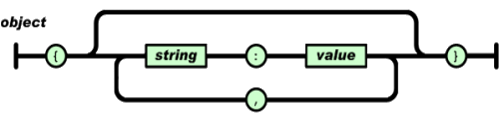
\includegraphics[width=120mm,height=25mm]{images/objectJSON}}
\caption{Object JSON} \label{fig:objectJSON}
\end{figure}

Un arreglo es una colecci\'on de valores. Un arreglo comienza con [ (corchete izquierdo) y termina con ] (corchete derecho). Los valores se separan por , (coma).

\begin{figure}[H]
\centering
\subfigure{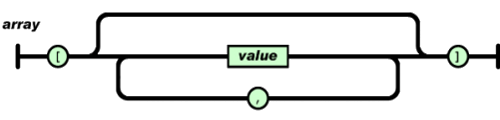
\includegraphics[width=120mm,height=25mm]{images/arrayJSON}}
\caption{Array JSON} \label{fig:arrayJSON}
\end{figure}

Un valor puede ser una cadena de caracteres con comillas dobles, o un n\'umero, o true o false o null, o un objeto o un arreglo. Estas estructuras pueden anidar

\begin{figure}[H]
\centering
\subfigure{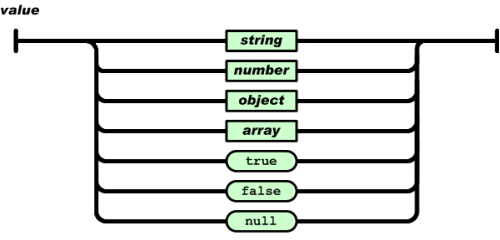
\includegraphics[width=120mm,height=65mm]{images/valueJSON}}
\caption{Value JSON} \label{fig:valueJSON}
\end{figure}

Una cadena de caracteres es una colecci\'on de cero o m\'as caracteres Unicode, encerrados entre comillas dobles, usando barras divisorias invertidas como escape. Un car\'acter est\'a representado por una cadena de caracteres de un \'unico car\'acter. Una cadena de caracteres es parecida a una cadena de caracteres C o Java.

\begin{figure}[H]
\centering
\subfigure{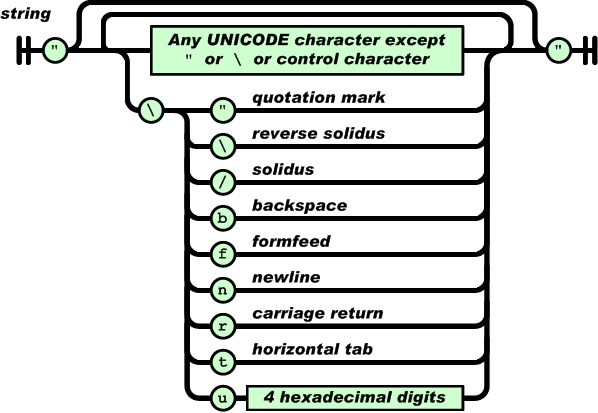
\includegraphics[width=120mm,height=60mm]{images/stringJSON}}
\caption{String JSON} \label{fig:stringJSON}
\end{figure}

Un n\'umero es similar a un n\'umero C o Java, excepto que no se usan los formatos octales y hexadecimales.

\begin{figure}[H]
\centering
\subfigure{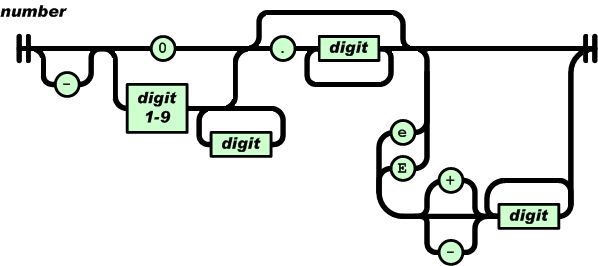
\includegraphics[width=120mm,height=50mm]{images/numberJSON}}
\caption{Number JSON} \label{fig:numberJSON}
\end{figure}

Los espacios en blanco pueden insertarse entre cualquier par de s\'imbolos.

\section{Persistencia de la informaci\'on de metadatos}
La informaci\'on obtenida en el anterior capitulo es necesario que sean persistentes para la reanudaci\'on  en el proceso de configuraci\'on para el objetivo, la informaci'on necesaria a persistir son las siguientes:
\begin{itemize}
\item Datos de la conexi\'on a la base de datos como ser el nombre de la base de datos, usuario, contrase\~na, puerto y el host.
\item La lista de las tablas de la base de datos elegida seg'un al orden en que estos deben ser llenados que obtuvimos en el capitulo anterior.
\item El detalle por cada una de las tablas (nombre de la columna, el tipo de dato, si acepta que sea nulo, si es una llave etc...).  
\end{itemize}
Una alternativa para dar soluci\'on a este requisito es almacenar toda esta informaci'on en archivos sea en el formato JSON o XML, en este proyecto se optar\'a por Json las razones son las siguientes:

\begin{itemize}
\item Soporta dos tipos de estructuras, una de ellas son objetos que contienen una colecci\'on de pares llave-valor y el otro tipo se trata de arrays de valores. Esto proporciona una gran sencillez en las estructuras.
\item No tiene espacios de nombres, cada objeto es un conjunto de claves independientes de cualquier otro objeto.
\item JSON no necesita ser extensible por que es flexible por s\'i solo. Puede representar cualquier estructura de datos pudiendo a\~nadir nuevos campos con total facilidad.
\item Es mucho mas simple que XML, el cual proporciona pesadas tecnolog\'ias que le avalan (Scheme, XSLT, XPath).
\item Si comparamos el tama\~no de un archivo JSON con uno XML y que contenga la misma informaci\'on el primero llega a ser mucho mas peque\~no.
\end{itemize} 
\subsection{Creando la estructura de un proyecto}
Cuando sea crea un proyecto java ,php , python etc... normalmente se tiene un estructura de directorios y archivos, donde ciertos archivos guardan configuraciones sobre recursos que se hacen uso, la version del proyecto entre otros. Para este proyecto realizaremos algo similar para lo cual se va tener como base la siguiente estructura de directorios y archivos

\begin{figure}[H]
\centering
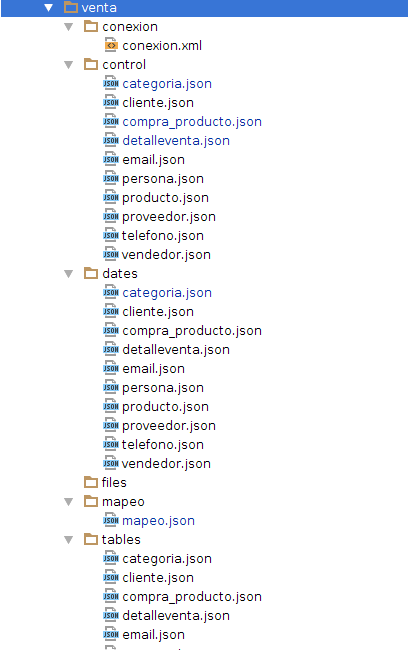
\includegraphics[scale=0.5]{images/estructura.png}
\caption{Estructura}
\end{figure}

Donde se guarda la informaci'on de los archivos de configuraci'on, veamos en detalle cada directorio y su contenido:
\begin{itemize}
\item \textbf{conexi\'on} En este directorio se tiene un archivo \textit{conexion.xml} la cual contiene la informaci'on de los datos de conexi'on. Va separada en un directorio por razones de que puede existir un nombre de una tabla igual al archivo por lo que es necesario que no se confunda.
\item \textbf{control} Si observamos el contenido de los directorios \textit{control,dates,tables} son similares la diferencia esta en el contenido de los archivos.
 
En este directorio almacenamos archivos de control de las columnas por cada tabla y que tienen el mismo nombre que en la base de datos veamos el contenido para la tabla \textit{compra\_producto} de la Figura \ref{fig:Modelo ER}.
\lstset{language=java,breaklines=true}
\label{tablaCompraProductoArchivoControl}
\captionof{lstlisting}{Ejemplo archivo control}
\begin{lstlisting}
[
  {
    "column_name": "cod_producto",
    "is_nullable": "NO",
    "rellenado": false
  },
  {
    "column_name": "cod_proveedor",
    "is_nullable": "NO",
    "rellenado": false
  },
  {
    "column_name": "cod_compra_producto",
    "is_nullable": "NO",
    "rellenado": false
  },
  {
    "column_name": "fecha_compra_producto",
    "is_nullable": "NO",
    "rellenado": false
  }
]
\end{lstlisting}.
 
Encontramos informaci\'on en formato JSON clave - valor y donde \textit{column\_name} indica el nombre de la columna, \textit{is\_nullable} nos indica si este campo puede ser nulo y por ultimo \textit{rellenado} llega a ser la mas importante porque es aqu'i donde controlamos si ya fue configurada esta columna.
\item \textbf{dates} los archivos de este directorio almacenan informaci'on generada por cada columna, a excepci'on de tipos de datos como bytea o blob, para este tipo de datos es recomendable almacenar el nombre del archivo. El formato del archivo que almacena la informaci\'on generada es el siguiente:
\lstset{language=java,breaklines=true}
\label{tablaCompraProductoArchivoControl}
\captionof{lstlisting}{Ejemplo archivo control}
\begin{lstlisting}
[
  {
    "nombre_categoria": "bebida",
    "cod_categoria": "1"
  },
  {
    "nombre_categoria": "comidarapida",
    "cod_categoria": 2
  },
  {
    "nombre_categoria": "enlatados",
    "cod_categoria": 3
  },
  {
    "nombre_categoria": "especial",
    "cod_categoria": 4
  },
  {
    "nombre_categoria": "ensaladas",
    "cod_categoria": 5
  }
]
\end{lstlisting}
Si observamos la Figura \ref{fig:Modelo ER} la tabla \textit{categoria} tiene dos atributos \textit{nombre\_categoria} y \textit{cod\_categoria}, si vemos el contenido del archivo \textit{categoria.json} de directorio \textit{dates} existen varios registros con los valores asignados, la cantidad puede variar dependiendo de la cantidad de datos que se quiere generar.
 \item \textbf{files} En este directorio se almacenan los archivos de tipo bytea y que al momento de hacer la insercion las usamos por su nombre.
 \item \textbf{mapeo} Solo existe un archivo con un contenido de la lista de las tablas seg'un el orden en que estas deben ser configurados adem'as tiene dos atributos mas \textit{nivel} la cual nos indica cual es el orden en que le corresponde y por ultimo la \textit{cantidad} si encontramos un valor igual a cero es porque esta tabla no tiene columna alguna configurada esto nos deja entender que si se da un valor, es para la tabla en general. Veamos para la el caso de la Figura \ref{fig:Modelo ER}
\lstset{language=java,breaklines=true}
\label{tablaCompraProductoArchivoControl}
\captionof{lstlisting}{Ejemplo archivo control}
\begin{lstlisting}
[
  {
    "tablename": "categoria",
    "nivel": 0,
    "cantidad": "5"
  },
  {
    "tablename": "persona",
    "nivel": 0,
    "cantidad": 0
  },
  {
    "tablename": "producto",
    "nivel": 1,
    "cantidad": 0
  },
  .
  .
  .
  {
    "tablename": "compra_producto",
    "nivel": 2,
    "cantidad": 0
  },
  {
    "tablename": "detalleventa",
    "nivel": 2,
    "cantidad": 0
  }
]
\end{lstlisting}  
\item \textbf{tables} En el directorio tables es donde almacenamos la informaci'on detallada por cada una de las tablas, adem'as cada archivo representa a una tabla de la base de datos y que llevan el mismo nombre. Veamos el contenido del archivo \textit{categoria.json} que representa a la tabla \textit{categoria}:
\lstset{language=java,breaklines=true}
\label{tablaCompraProductoArchivoControl}
\captionof{lstlisting}{Ejemplo archivo control}
\begin{lstlisting}
[
  {
    "column_name": "cod_categoria",
    "data_type": "integer",
    "character_maximum_length": null,
    "es_foranea": "false",
    "referencian": null,
    "tabla": null,
    "referenciados": null,
    "numeric_precision": "32",
    "is_nullable": "NO",
    "constraint_type": "PRIMARY KEY",
    "column_default": "nextval('categoria_cod_categoria_seq'::regclass)",
    "check_clause": null
  },
  {
    "column_name": "nombre_categoria",
    "data_type": "character varying",
    "character_maximum_length": null,
    "es_foranea": "false",
    "referencian": null,
    "tabla": null,
    "referenciados": null,
    "numeric_precision": null,
    "is_nullable": "NO",
    "constraint_type": null,
    "column_default": null,
    "check_clause": null
  }
]
\end{lstlisting} 
\end{itemize}

Es una estructura de directorios que no necesariamente se tienen que llamar as'i, sin embargo el nombre de los archivos es aconsejable que lleven el mismo nombre que en la base de datos para que resulte mas amigable.
\section{Configuraci'on de columnas}
Una vez que se tiene el proyecto creado, la configuraci'on que se hace es por cada columna de la tabla para lo cual necesitamos saber que tipo de dato acepta cada columna o si hace referencia a otra tabla.
Las columnas de una tabla puede ser de diferente tipo de dato(\textit{integer, varchar, boolean etc...}. Independientemente del tipo de dato de una columna se puede agruparlos tomando en cuenta ciertas caracter'isticas como ser:
\begin{itemize}
\item Que el tipo de dato sea texto, fechas hora, direcciones de red al momento de insertar a la base de datos estos son tomados como si fuesen un texto($'$\textit{valor}$'$).
\item El tipo de dato sea un numero en las que estan (\textit{integer,serial,smallserial,bigserial, beint ...smallint}) est'an son insertados como un numero (\textit{valor}).
\item Que sea una llave primaria sin importar el tipo de dato est'an deben ser 'unicas al momento de generarlos.
\item Cuando sea una llave for'anea no se debe generar por que estas deben existir en la tabla que hace referencia para lo cual se toma los valores generados en la tabla referenciada.
\item El tipo de dato sea bytea es un caso especial que no se trata como una cadena ni como un numero.
\end{itemize}
\subsection{Configuraci'on para llaves for'aneas}
Las llaves for'aneas o primarias que no son propias de la tabla no se necesitan generarlos con un algoritmo, lo que se hace es trabajar con los datos generados en la columna de la tabla al que se hace referencia, En este proyecto la t'ecnica empleada para el manejo de estas fue agruparlos todas las que hacen referencia en conjunto a alguna tabla como si fuese una sola columna veamos un ejemplo
\begin{figure}[H]
\centering
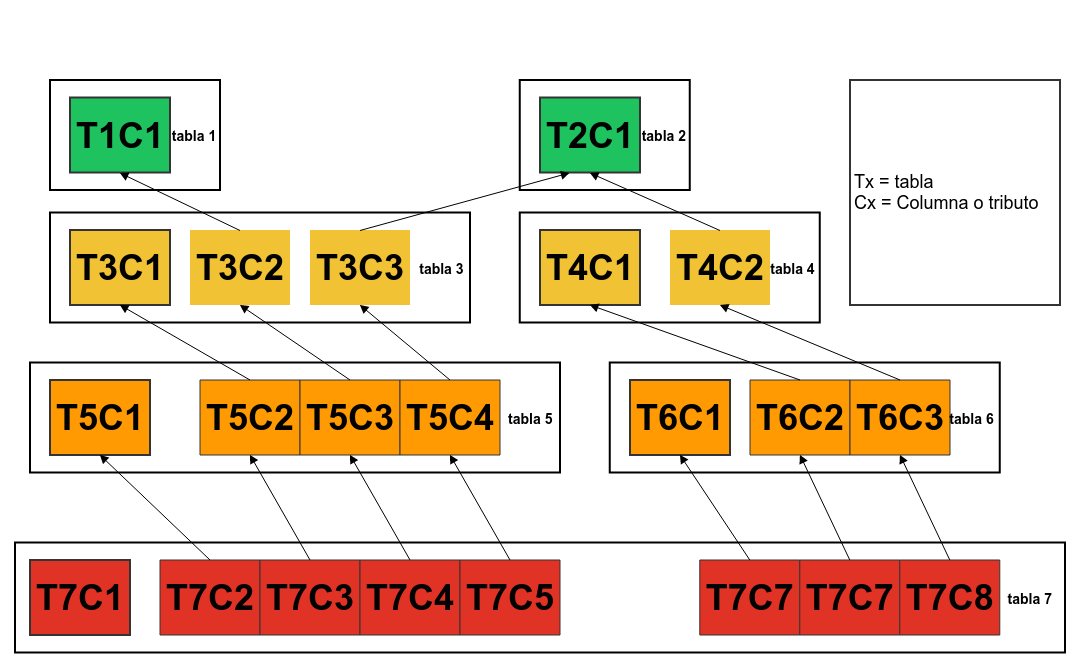
\includegraphics[scale=0.4]{images/foraneasline.png}
\caption{Foraneasline}\label{fig:ejemploForaneasLine}
\end{figure}
En la Figura \ref{fig:ejemploForaneasLine} la \textit{tabla1} cuenta con una llave primaria (\textit{T1C1})  al igual que la \textit{tabla2}, y si bajamos un nivel mas abajo a la \textit{tabla3} esta hace referencia a \textit{tabla1} y \textit{tabla2} y que las columnas de las tablas referenciadas mandan como llaves primarias, formando asi una llave compuesta para \textit{tabla3}.Por otro lado la \textit{tabla4} hace referencia a \textit{tabla2} y que tambie tiene una llave compuesta. Si bajamos a la \textit{tabla5} esta compuesta de 4 columnas de las cuales 3 no son propias, si nos fijamos vienen juntadas como si fuera una columna es lo que hicimos al momento de guardar el detalle de una tabla, En la \textit{tabla7} se hace referencia a la \textit{tabla5} y \textit{tabla6} y las columnas que no son propias son agrupadas de acuerdo a que tabla se haga referencia es el caso de \textit{T7C2,T7C3,T7C4,T7C5} que en conjunto hacen referencia a la \textit{tabla5} y \textit{T7C6,T7C7,T7C8} hacen referencia a \textit{tabla6}.

Al momento de hacer la configuraci\'on llegamos a tener un problema, de la \textit{tabla5} el campo  \textit{T5C2,T5C3,T5C4} no lo encontramos si lo buscamos como una columna en la \textit{tabla3} como es posible si tenemos esas columnas? Es cierto que existen pero est'an separadas
\begin{figure}[H]
\centering
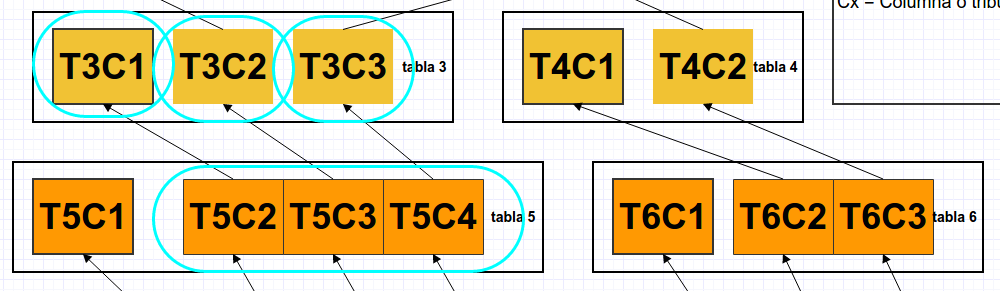
\includegraphics[scale=0.4]{images/problemaColumnas.png}
\caption{Problema llaves foraneas}\label{fig:problemaColumnasForaneasLine}
\end{figure}
Como se observa en la Figura \ref{fig:problemaColumnasForaneasLine} se da el mismo problema para la \textit{tabla7} la columna \textit{T7C2,T7C3,T7C4,T7C5} no se encuentra en una solo columna en la \textit{tabla5} pero hay algo interesante que se puede deducir veamos la siguiente figura:
\begin{figure}[H]
\centering
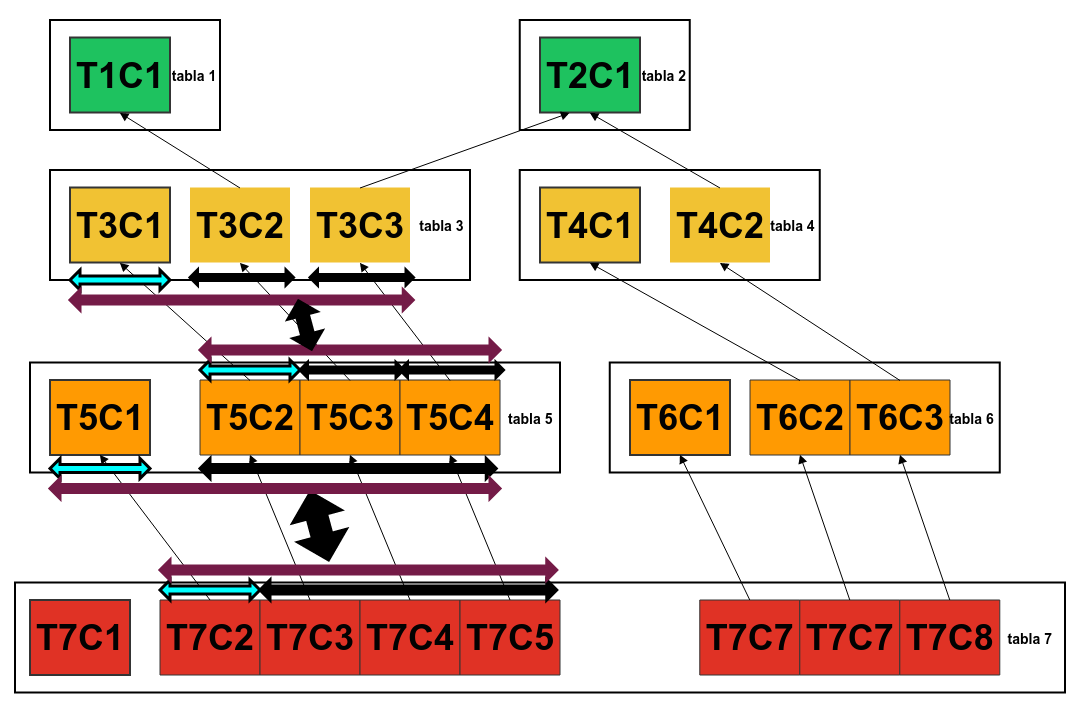
\includegraphics[scale=0.3]{images/problemaForaneas.png}
\caption{Ejemplo foraneas unidas}\label{fig:problemaColumnasForaneasGrafica}
\end{figure}
En la \textit{tabla5} las columnas \textit{T5C2,T5C3,T5C4} en conjunto hacen referencia como una sola a la \textit{tabla3} donde \textit{T5C2} apunta a \textit{T3C1} y que esta es una llave primaria propia de la \textit{tabla3}, si vamos a la \textit{tabla7} la columna  \textit{T7C2} hace referencia a una propia de la \textit{tabla5}, Podemos determinar que el comportamiento de las llaves primarias que no son propias siguen este modelo.
\subsubsection{Problemas}
El problema surge al momento de realizar la validaci\'on que por ejemplo cuando por alguna raz\'on tratamos de configurar un atributo que hace referencia y que previamente no se configur\'on los atributos referenciados en la tabla referenciada no se llega a encontrar como se ve en la figura \ref{fig:problemaColumnasForaneasGrafica}. Las columnas de la \textit{tabla3} se van encontrar todas al igual que en la \textit{tabla4}, pero en la \textit{tabla5} no se llega a encontrar la columna \textit{T5C2T5C3T5C4} lo mismo sucede con \textit{T6C2T6C3}.
Una vez hecha la validaci\'on el siguiente paso es configurar, para lo cual se necesita los datos de la tabla referenciada, y nos fijamos en la Figura \ref{fig:problemaColumnasForaneasGrafica} nos encontramos en el mismo problema de la validaci\'on de columnas no encontradas.   
\subsubsection{Soluci\'ones}
Una soluci\'on obvia al problema de la validaci\'on presentado es verificar que todas las columnas de la tabla referenciada se encuentren configuradas para no tener problemas al obtener los datos pero no es tan cierto se puede configurar con solo tener configuradas las columnas referenciadas podemos optar por cualquiera son cuestiones de validaci\'on.

En cuanto al problema de la configuraci\'on una vez pasada la anterior la soluci\'on no llega a ser tan sencilla necesitamos aplicar algun mecanismo(os) de obtener los datos, La soluci\'on que damos no estrictamente as'i depende del modelo y del manejo de llaves
\begin{figure}[H]
\centering
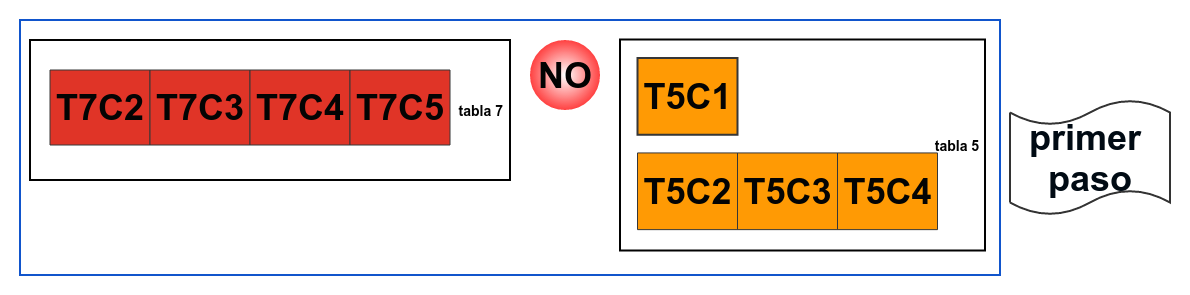
\includegraphics[scale=0.35]{images/paso1.png}
\caption{Intento 1}\label{intento1}
\end{figure}
En el intento 1 no llegamos a la soluci\'on ya que no encontramos la columna en la \textit{tabla5}
\begin{figure}[H]
\centering
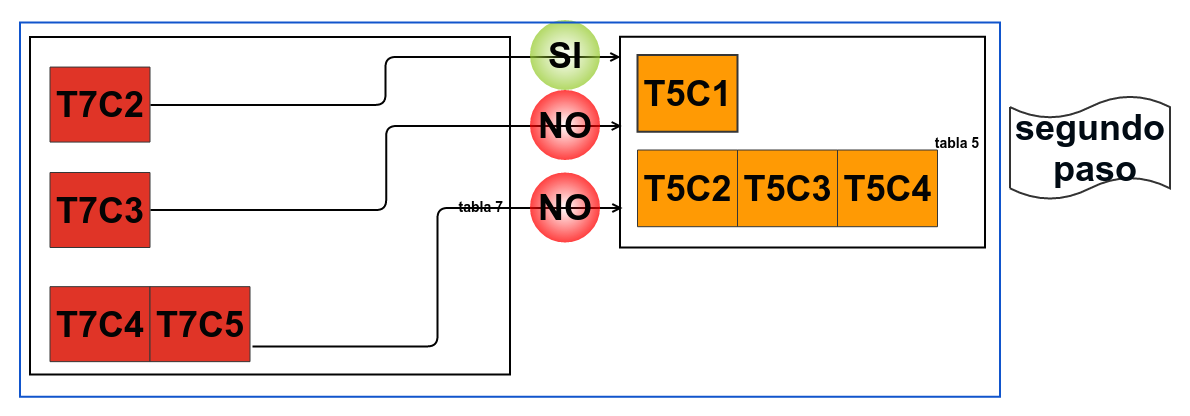
\includegraphics[scale=0.35]{images/paso2.png}
\caption{Intento 2}\label{intento2}
\end{figure}
Iniciamos con el primer elemento buscando en la tabla referenciada en caso de que exista pasamos al siguiente elemento caso contrario listamos en una lista de los elementos no encontrados
\begin{figure}[H]
\centering
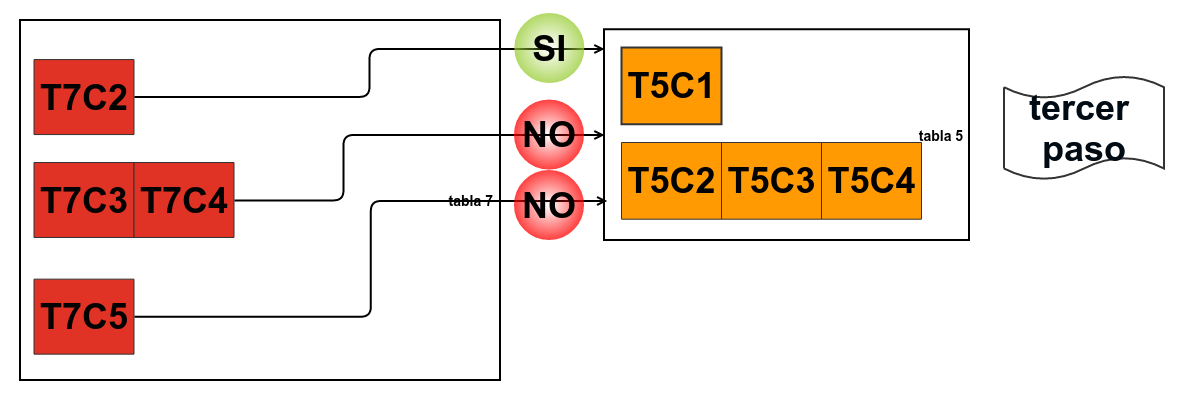
\includegraphics[scale=0.35]{images/paso3.png}
\caption{Intento 3}\label{intento3}
\end{figure}
Pasamos con el siguiente elemento uniendo con las no encontradas y volvemos a buscar en la tabla referenciada como aun no encontramos pasamos al siguiente
\begin{figure}[H]
\centering
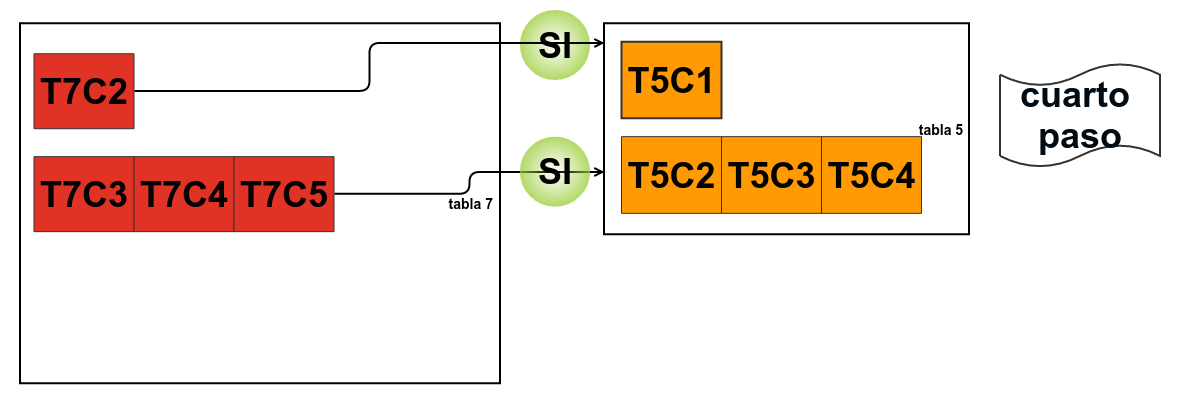
\includegraphics[scale=0.35]{images/paso4.png}
\caption{Intento 4}\label{intento4}
\end{figure}
En este paso volvemos a juntar las no encontradas y el elemento a obtener y buscamos en la tabla referenciada y como encontramos y no hay mas elementos que buscar se llega a la soluci\'on